%!TEX root = ../thesis.tex
\define{\imgpath}{french/img}

\chapter*{Résumé substantiel}
\label{chapter:frecnhresume}
\minitoc

Suivre l'organisation de l'abstract. Faire plien de référence au chapitre de la thèse.

\subsection*{Introduction}

Problème de l'intéraction humain-machine.

Pour interagir il faut que la machine comprenne le sens des signaux de communication de l'humain.

Pour apprendre le sens des signaux,  il faut savoir ce que l'humain veut dire pour construire un modèle statistique des signaux.

Dans cette thèse nous étudions comment il est possible de créer des interfaces ne nécessitant pas de phase de calibration.

facilemet transposable a dautre signaux, parole: pas d'apriori sur le sens des mots

\subsection*{Etat de l'art}

Tres peu de travaux s'interresse a cette question. 

Et il est interressant de voir que c'est la communaute BCI qui s'est interresse le plus à ce problème. En effet, a l'opposé des mode d'interaction classique, telle que la parole, les gestes, ou les expression faciale, nous n'avons aucun apriori sur l'utilisation des signaux du cerveau. Le problème de l'auto-calibration est alors plus flagrant dans le domaine des BCI. 

Les travaux de Peter Jan Kindermans sont les plus proche de nos travaux. 

\subsection*{Principe algorithmique}

Pour cela, nous allons mettre en place un système d'hypothèse sur la tâche que veut effectuer l'utilisateur. Et créer autant d'interpretation que de tâche possible. Notre hypothèse sous-jacente est que seule l'hypothèse correcte, i.e. celle suivi par l'utilisateur vera une cohérence entre les labels assignés aux données et la structure de ces données dans l'espace de features.

le planning est égelemtn différent des algortihmes précedemment dévellopé. En effet une couche d'incertitude supplémentaire est présente, le sens des signaux est inconnue et nous disposont d'une multitude de candidat possible. Il faut donc inclure cette incertitude dans la mesure d'incertidtude globale permettant de naviguer plus efficacement dans le monde. afin de collecter des signaux varié. 

As mentioned before, in this work the robot cannot rely on the phase of calibration. However the robot has access to the interaction frame, which provides theoretical information about the human teaching behavior. The robot knows:
\begin{itemize}

\item \textbf{Details and timing of the interaction.} After each action, the robot waits for a signal from the teacher. This signal provides information related with the action the robot just performed.

\item \textbf{The set of possible meanings the human can refer to.} The teacher assesses the last action of the robot with respect to an unknown task. The signals' meanings can be ``correct'' or ``incorrect''.

\item \textbf{Constraints on the possible tasks.} There are only two possible tasks, reaching the left (G1) or the right (G2) edge of the T world.

\end{itemize}

In addition the robot has access to the $Frame(Context,Task)$ function that, given a context of interaction and a task, returns the meaning intended by the teacher. For example, the robot knows that if it moves from state 3 to state 2, and that the human wants it to go in G1, then the signals received from the human means ``correct''.


For each action, the robot receives raw unlabeled two dimensional signals. Following the above explanation, for a particular hypothesis (G1 or G2), the robot can assign hypothetic meanings to the human signals knowing they are limited to a finite set and according to the interaction history. We assume our teacher is optimal and therefore assume our agent is aware of the optimal policies for each task  (see Figure~\ref{fig:Twolrdpolicies}), which can be used to interpret the human signals.

% The machine is ``reasoning'' as follow: \emph{"If the human wants me to solve task G1 then when I performed action $a$ in state $a$ and he said ``oui'', he meant ``incorrect''"}. 

% We exemplify this process using the same example as in Figure~\ref{fig:TworldOneStepUnlabeled} and according to our two task hypothesis which are reaching either of the two edges marked as G1 or G2. 

\begin{figure}[!htbp]
  \centering
  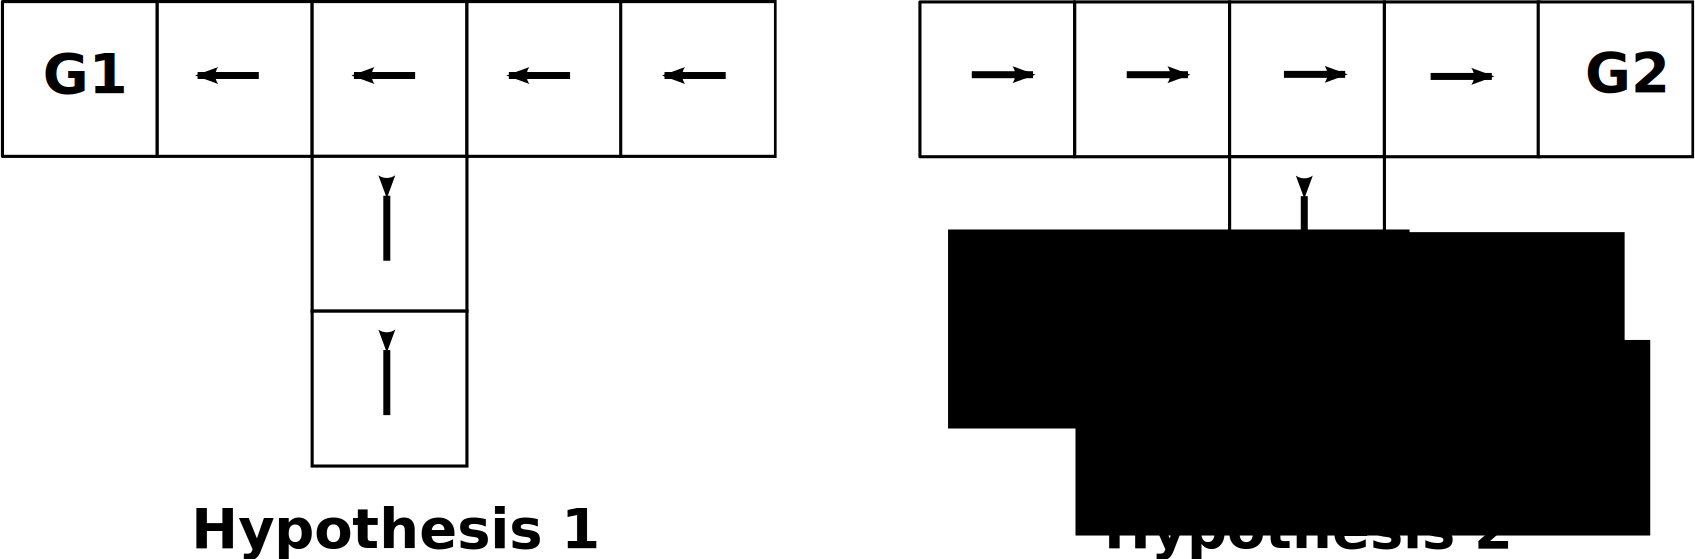
\includegraphics[width=\tworldsize\columnwidth]{\visualspdf/tuto_feedback/Tworld_hypothesis.pdf}
  \caption{Optimal policies associated to the two task hypotheses G1 and G2 in the T world. Such policies are known by both the human and the agent, and allow the agent to interpret a human signal with respect to a given task.}
  \label{fig:Twolrdpolicies}
\end{figure}

The teacher wants the agent to go to G1. The agent starts in state 3, performs action left, and ends-up in state 2. The teacher sends a signal in the right part of the feature space, meaning that the previous action was ``correct''. However the agent does not have access to the label associated to this signal and it only observes a point in a two dimensional space (Figure~\ref{fig:TworldLabelunknown}). The agent generates interpretation hypothesis according to G1 and G2. With respect to G1, the action was ``correct'' (Figure~\ref{fig:TworldLabelG1}), while with respect to G2 the action was ``incorrect'' (Figure~\ref{fig:TworldLabelG1}).

\begin{figure}[!htbp]
    \centering
    \begin{subfigure}[b]{\tworldsize\columnwidth}
        \centering
        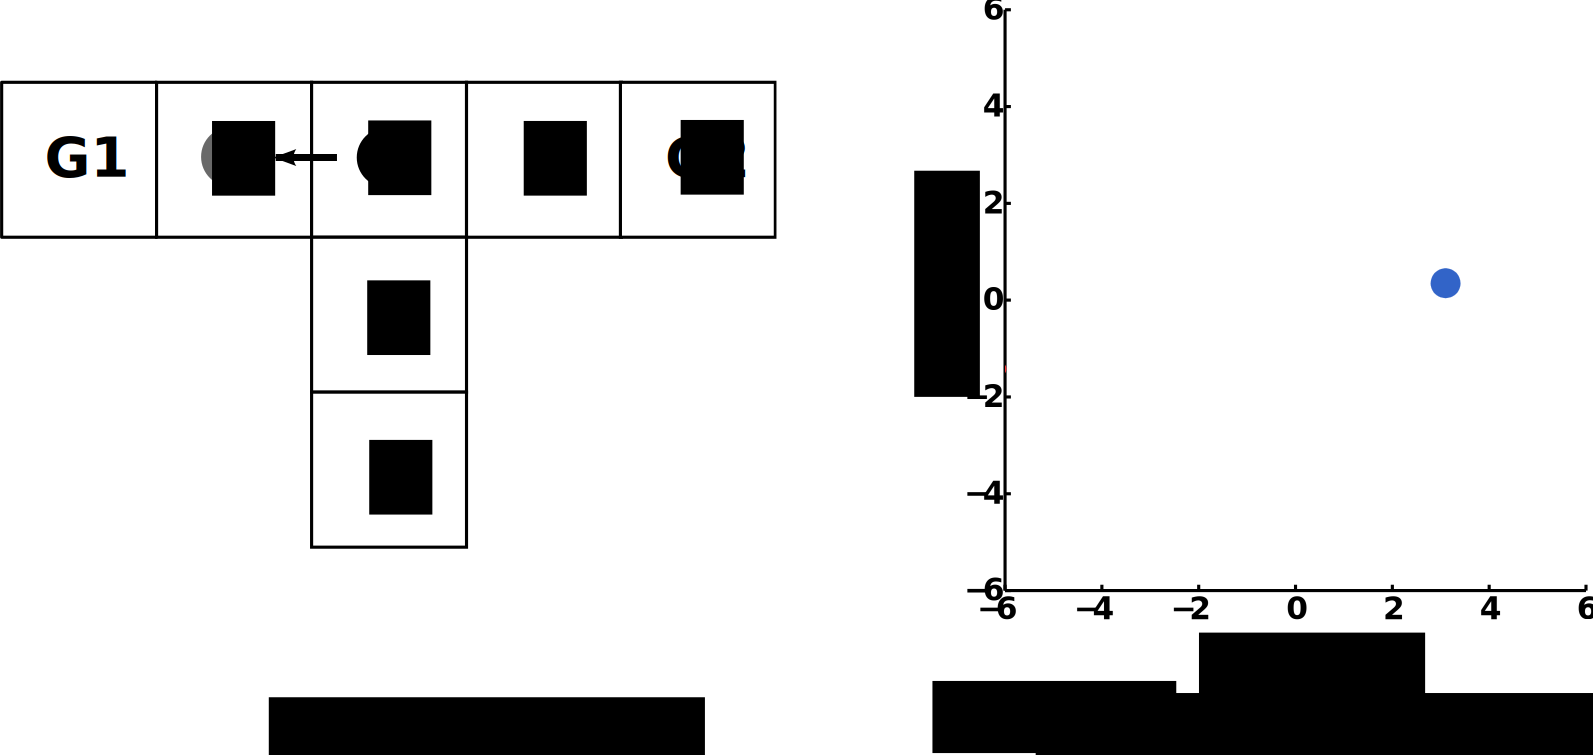
\includegraphics[width=\columnwidth]{\visualspdf/tuto_feedback/Tworld_feedback_unlabeled_one_action.pdf}
        \caption{Feedback signal as received by the agent without label.}
        \label{fig:TworldLabelunknown}
    \end{subfigure}\\
    \begin{subfigure}[b]{\tworldsize\columnwidth}
        \centering
        \includegraphics[width=\columnwidth]{\visualspdf/tuto_feedback/Tworld_feedback_labeled_G1.pdf}
        \caption{Feedback signal labeled according to G1.}
        \label{fig:TworldLabelG1}
    \end{subfigure}
    \begin{subfigure}[b]{\tworldsize\columnwidth}
        \centering
        \includegraphics[width=\columnwidth]{\visualspdf/tuto_feedback/Tworld_feedback_labeled_G2.pdf}
        \caption{Feedback signal labeled according to G2.}
        \label{fig:TworldLabelG2}
    \end{subfigure}
    \caption{Interpretation hypothesis made by the agent according to G1 (\ref{fig:TworldLabelG1}) and G2 (\ref{fig:TworldLabelG2}). The agent starts in state 3, performs action left, and ends-up in state 2. The meaning of the signal is different for both hypotheses.}
    \label{fig:TworldLabelOneStep}
\end{figure}

By repeating this process for several iteration steps, with the agent taking random actions, the system end-up with a set of possible interpretation of the human teaching signals (see Figure~\ref{fig:TworldLabelinterpretation}). But as the user has only one objective in mind, in our case G1, only the correct interpretation will assign the correct labels to the observed signals. We say that the corresponding hypothesis exhibit a coherence between the signals and their associated meanings. 

\begin{figure}[!htbp]
    \centering
    \includegraphics[width=\tworldsize\columnwidth]{\visualspdf/tuto_feedback/Tworld_feedback_labeled_all_actions.pdf}
    \caption{Interpretation hypothesis made by the agent according to G1 and G2 after many interaction steps. The teacher's task is to have the agent reach G1. The agent is exploring all the state space randomly. The labels associated to the task G1 are more coherent with the spatial organization of signals in the feature space.}
    \label{fig:TworldLabelinterpretation}
\end{figure}

Part of the \emph{learning from unlabeled interaction frames} problem defined in chapter~\ref{chapter:introduction:lfui} is the assumption that the user is coherent and uses always the same kind of signal for the same meaning. By visual inspection, we can infer that hypothesis G1 is the correct one as the resulting mapping between signal and meaning is more coherent. The key challenge is to find out how to identify coherence between the spatial organization of signals in the feature space and their associated labels with the tools available to the robot, i.e. algorithmically. 

We will formalize this idea in section~\ref{chapter:lfui:how}. Before that, we add two comments to this section and we summarize all the underlying assumptions of our problem in section~\ref{chapter:lfui:assumptions}.

\subsection*{Résultats}

Nous demontrons plusieurs applications possible à nos algortihm de d'auto-calibration. L'interaciton homme-robot et l'interactin cerveau-machine. 

Nottre aprochce est tres generique et permet de commencer a interagir avec une machine pour la résolution du tache sequentiel sans cque le systeme comprenne par avance les signaux de communiatins e l'utilisateur. Ces signaux peuvent etre de differente type, vocaux, gestes, onde cerebrale et doivent pouvoir être représenté sous la forme d'un vecteur.


Au chapitre bci, nous présentons l'application principale de ce travail au interface cerveau-machine. Ce genre d'interface permet au personne a fort handicap d'interagir avec le monde exterieur par le bias de son cerveau. Plus precisement, nous pouvons enregistrer des varitions de potentiel à la surface du cerveau. Ces ondes ont des porpritété différent en fonction de l'activité mentale du sujet et il est possible de différentier des activité motrice et même des signaux d'erreur de type oui/non. Le problème de ces systeme est qu'ils ne sont pas universelle et doivent être adapté à chaque utilisateur. Ceete adaptation est faite par une periode de calibration ou l'utilisateur, souvent ennuyeuse, et durent laquelle le systeme est inutilisable et neccessitant l'intervention d'une personne exterieur. De plus, cette pahse de calibration doit être effectué régulièrmeent car les signaux varie de jour en jour. Mais aussi pas example lapossition du casqua EEG, necessitant une calibration quotidienne de ce genre d'interfcae. 


Nous avons appliqué nos algortihm d'auto-calibration au interface cerveau utilisateur, testé en simulation mais aussi avec de vrai patient. Nos résultats montre que notre approche est fonctionnelle et permet une utilisation pratique  de l'interface plus rapidement. De plus notre systemem ne necessite pas la presence d'une perosnne exterieur pour la pahse de calibraiton et est donc un candidat potentiel pour ammener l'utilisation des interface cerveau mahcine dans les maisons.

Nous donnaons ici un bref résumé de l'experience BCI aisni que les résultats majeurs.

Description de la tache BCI

\subsection{The visual navigation task}

The setup of our online experiment is shown in Figure~\ref{fig:BCIsetup}. A human subject is equipped with an EEG cup is facing a screen where is displayed a two dimensional grid. The grid is composed of 25 discrete states, 5 rows and 5 columns. In green is displayed an agent that is able to move in the four cardinal direction (N/S/E/W). In red is the target the user selected. The user will mentally assess each agent's action a being ``correct'' or ``incorrect'' with respect to the target location.

\begin{figure}[!htbp]
\centering
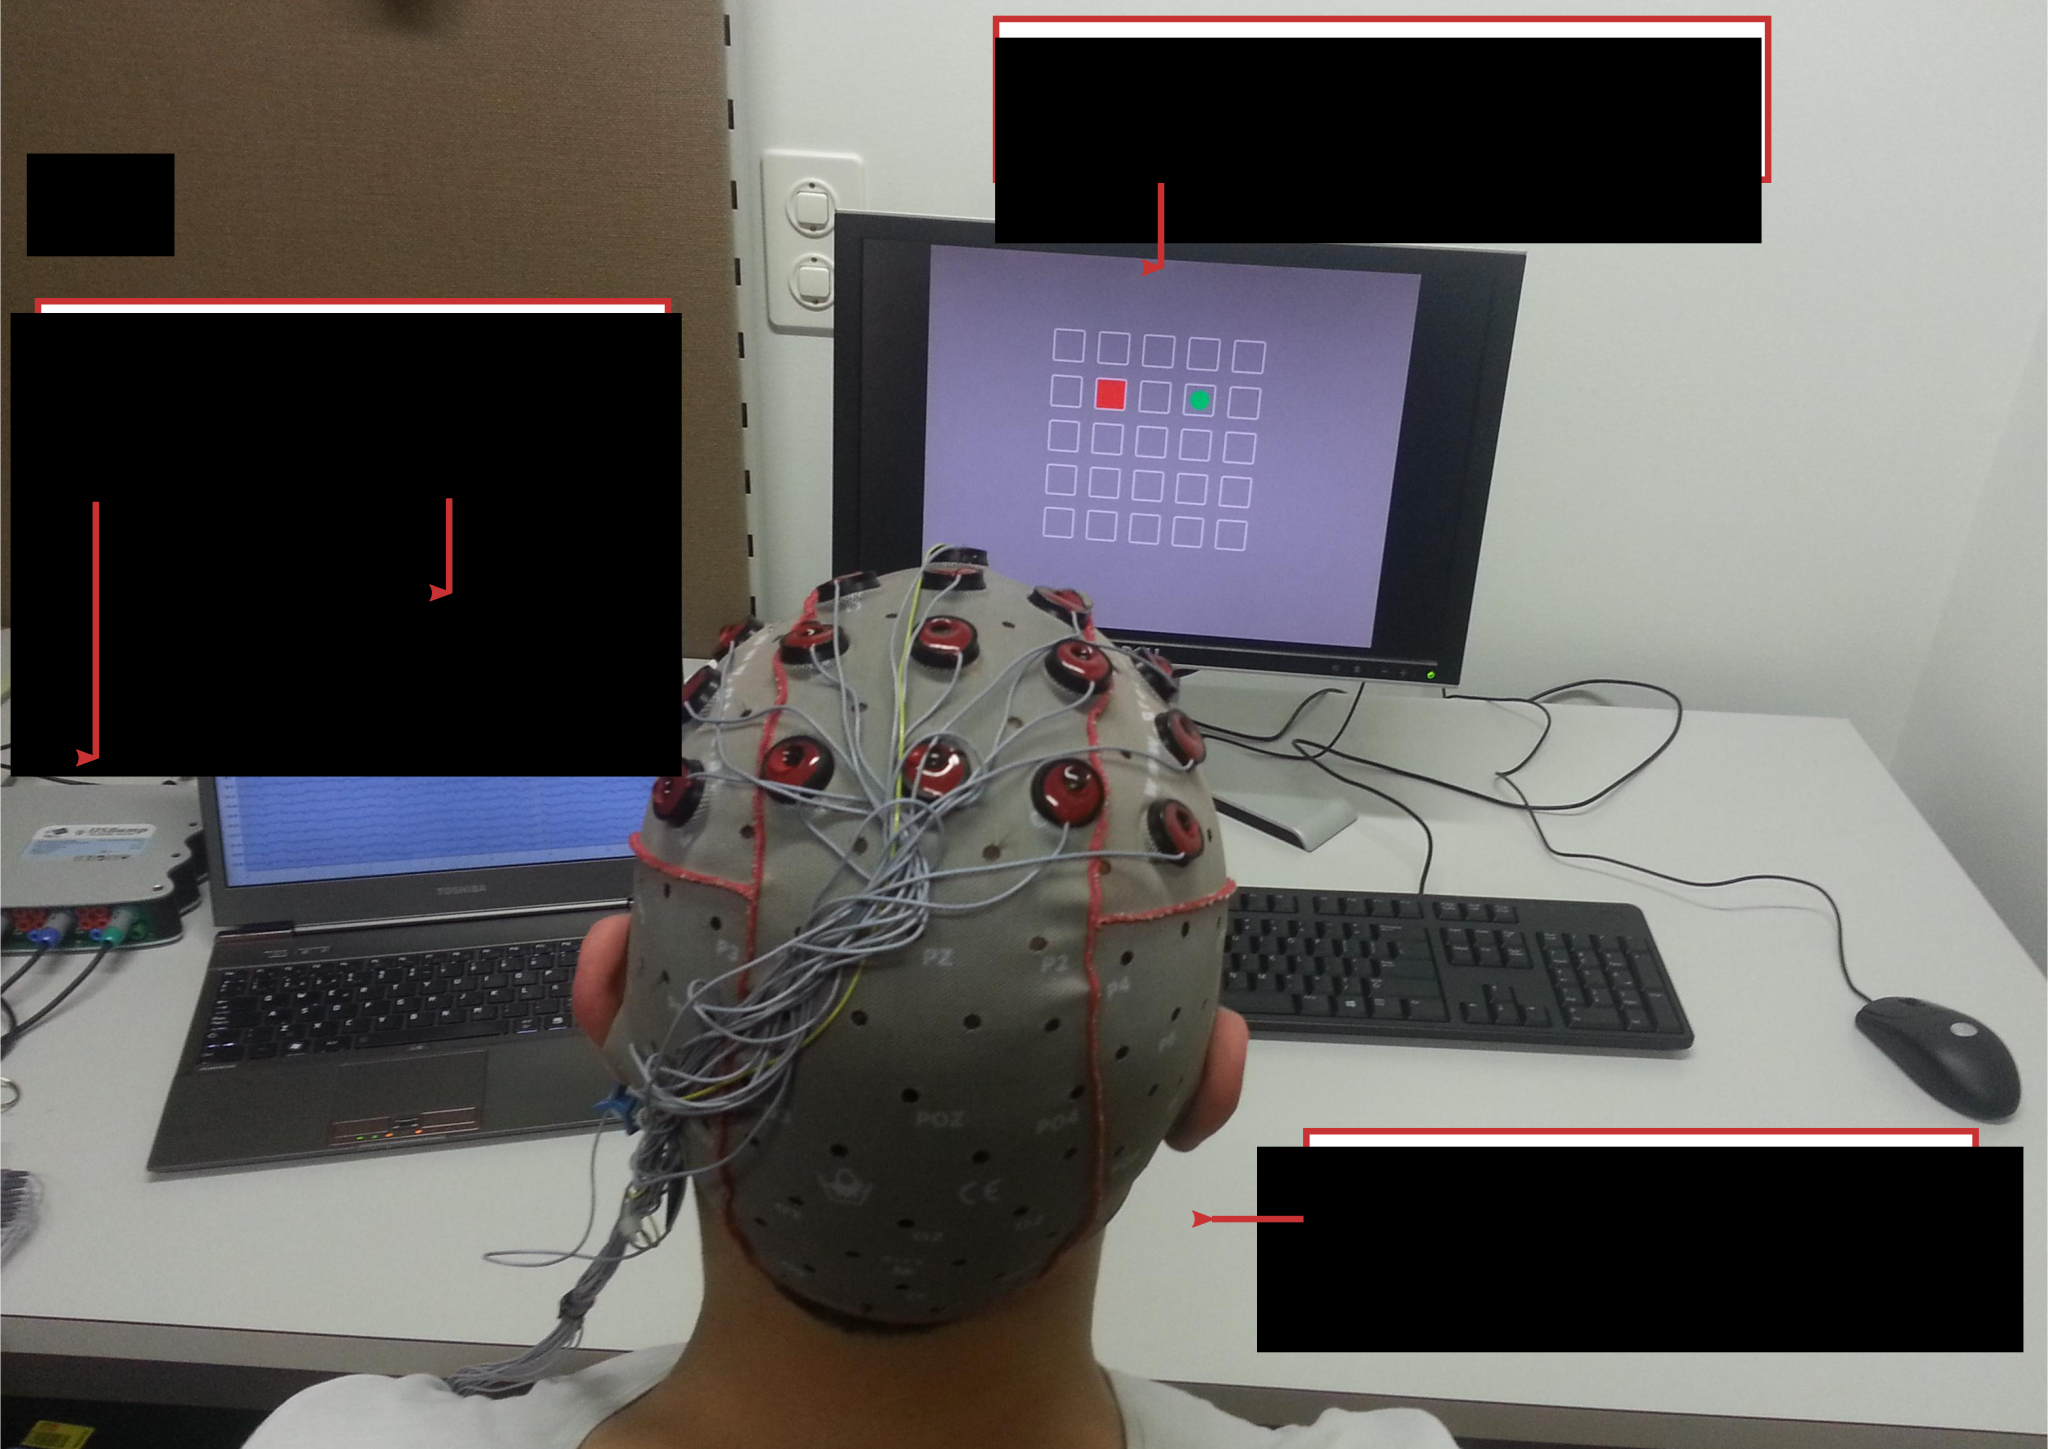
\includegraphics[width=\bcisetupsize\columnwidth]{\visualspdf/onlineXP/setup.pdf}
\caption{The BCI setup for online experiments. On the screen is displayed the grid world with the agent in green. We displayed the intended target in red, which was selected randomly. The purpose of this red square is to help the user remembering the target and our algorithm is at no point aware of the position of this red square.}
\label{fig:BCIsetup}
\end{figure}

\subsection{The brain signals}

We are interested by error-related potentials (ErrPs) in the subject's brain activity. These potentials are a specific kind of event-related potential (ERP) generated in the user's brain after s/he assesses actions performed by an external agent \cite{chavarriaga2010learning}. Correct and erroneous assessments will elicit different brain signals. As shown in Figure~\ref{fig:EEGsample}, the EEG signals associated to ``incorrect'' labels have slightly more amplitude than the one associated to ``correct'' labels, especially at around 350ms.

\begin{figure}[!htbp]
\centering
\includegraphics[width=0.49\columnwidth]{\imgpath/eeg_correct.eps}
\includegraphics[width=0.49\columnwidth]{\imgpath/eeg_incorrect.eps}
\caption{Low-pass filtered EEG signals associated to ``correct'' labels (left) and to ``incorrect'' labels (right). The signals for each class have slightly different amplitudes, especially at around 300ms.}
\label{fig:EEGsample}
\end{figure}

Past approaches have already demonstrated that these signals can be classified online with accuracies of around 80\% and translated into binary feedback, thanks to a prior calibration session that lasts for 30-40 minutes \cite{chavarriaga2010learning, iturrate2013task}.

time line

Figure~\ref{fig:sequence} shows one particular run of 500 steps comparing our self-calibration method with a calibration procedure of 400 steps. The two independent runs use a real EEG dataset with $80\%$ ten-fold cross-validation classification accuracy. As our algorithm is operational from the first step, it can estimate the real task when sufficient evidences have been collected. On the other hand, a calibration approach collects signal-label pairs for a fixed number of steps, and use the resulting classifier without updating it. This provokes that, during the calibration phase, no tasks can be learned, substantially delaying the user's online operation. 

Of important interest is the ability of the algorithm to evaluate when sufficient evidence has been collected. The dataset considered is of relatively good quality, and we do not need 400 steps to identify the first task. When doing a calibration procedure, the experimenter cannot know in advance the quality of each particular subject. Therefore, he must run a calibration for long enough so as to have enough examples to adapt to differences in signals' quality. 

% However, for some subject collecting 100 samples is enough.

\begin{figure}[!htbp]
\centering
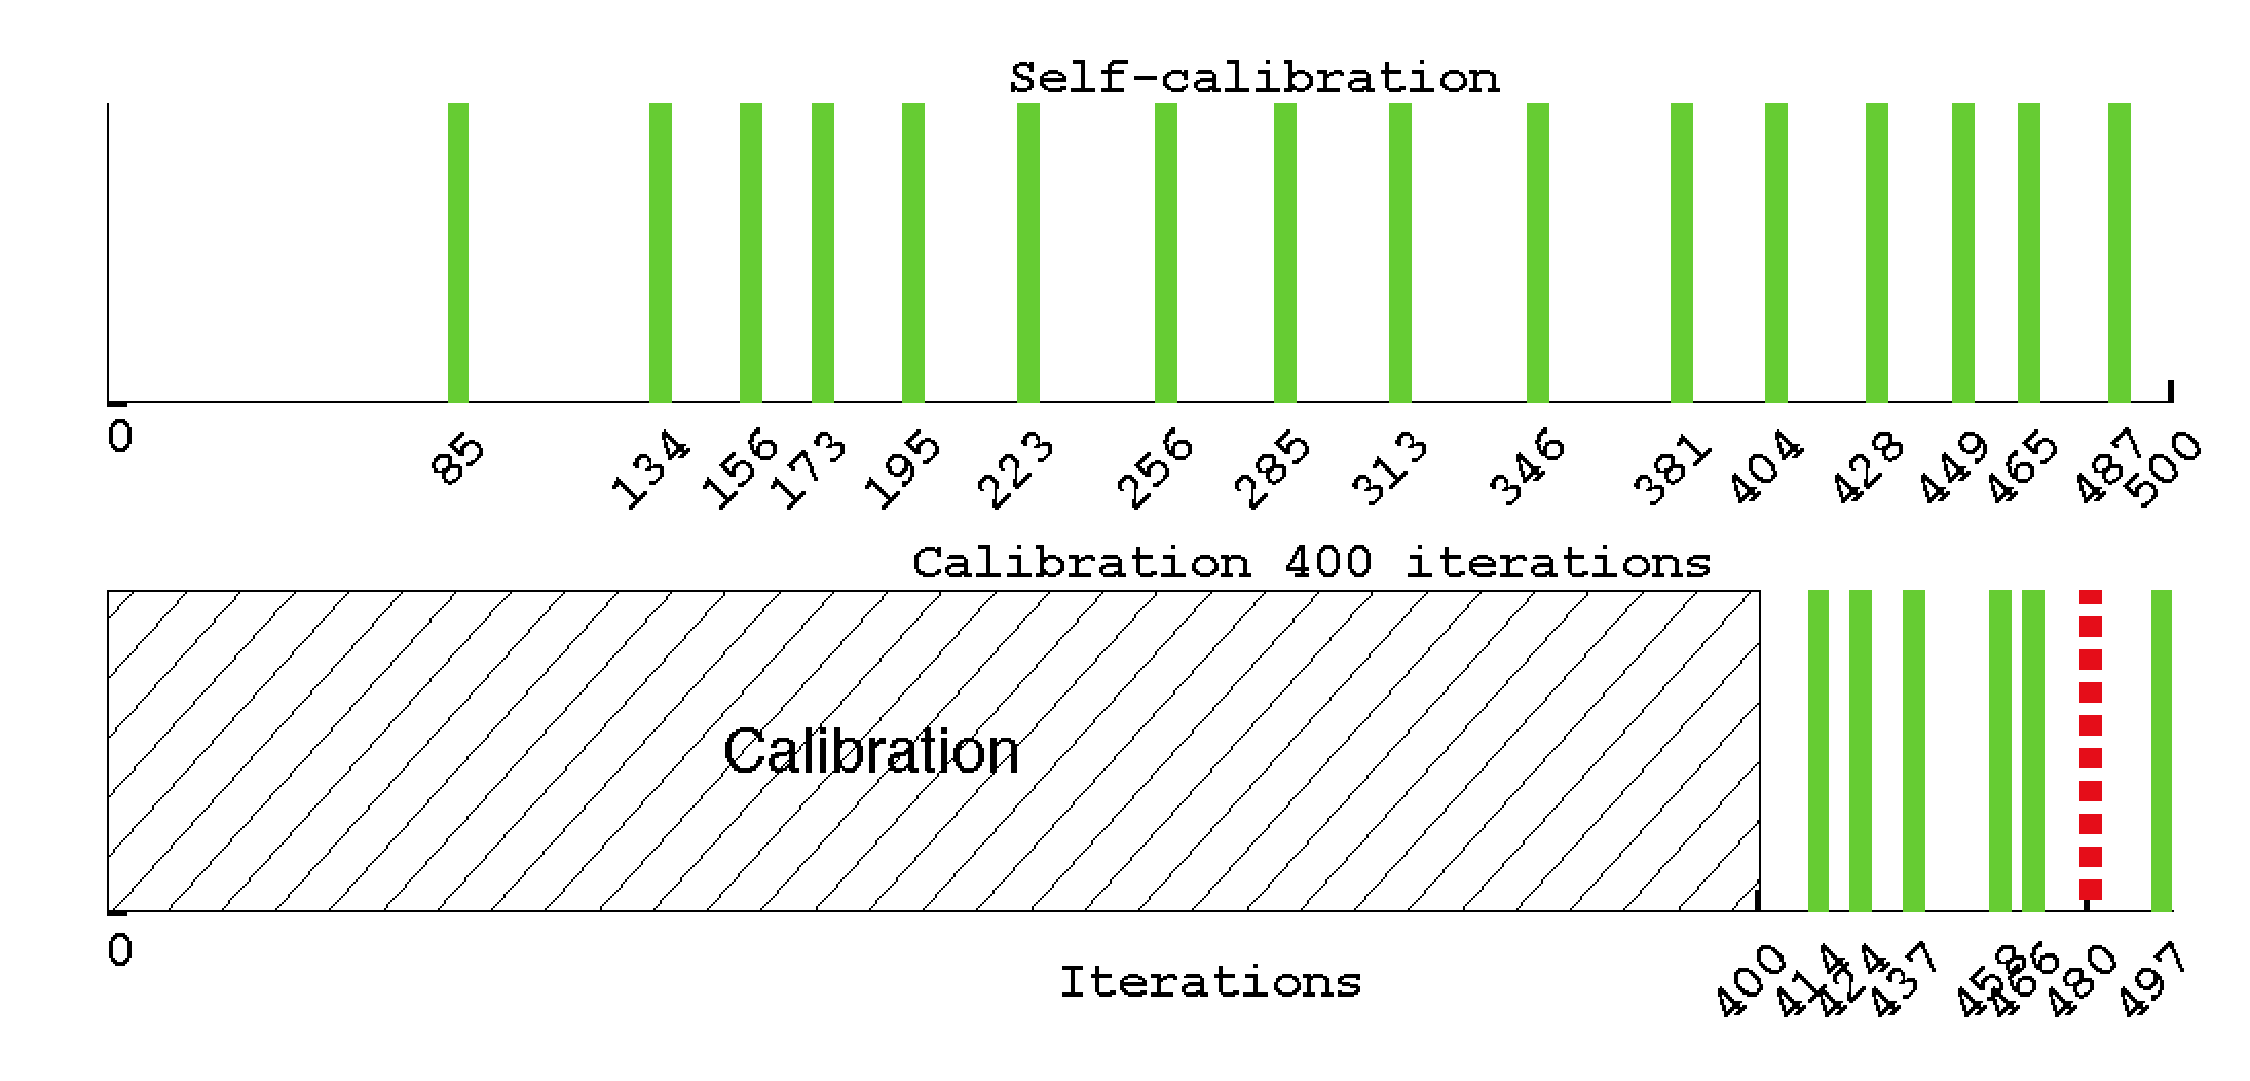
\includegraphics[width=\sequencesize\columnwidth]{\imgpath/plot_the_aaai_sequence.eps}
\caption{Timeline of one run using an EEG dataset of $80$ percent ten-fold cross-validation classification accuracy. Self-calibration (top) versus 400 steps calibration (bottom). Green (filled) and red (dashed) bars represent respectively correct and incorrect task achievements. The proposed self-calibration method allows reaching a first task faster than it takes to run a calibration procedure.}
\label{fig:sequence}
\end{figure} 


resultat avec des vrai sujet en temps réel

\begin{figure}[!htbp]
\centering
\includegraphics[width=\plotsize\columnwidth]{\imgpath/correct_and_error.eps}
\caption{Number of tasks correctly (green dot) and incorrectly (red crosses) achieved in 500+ steps during our online experiments with real subjects. We kept running the experiments after 500 steps until the systems identified the next task. The results are plotted against the a posteriori computed 10-fold accuracy of our classifier on each subject EEG signals. The performance of the system is correlated with the quality of the EEG signals. These results matches well with the results from simulated experiments.}
\label{fig:correcterror_online}
\end{figure} 


\begin{figure}[!htbp]
\centering
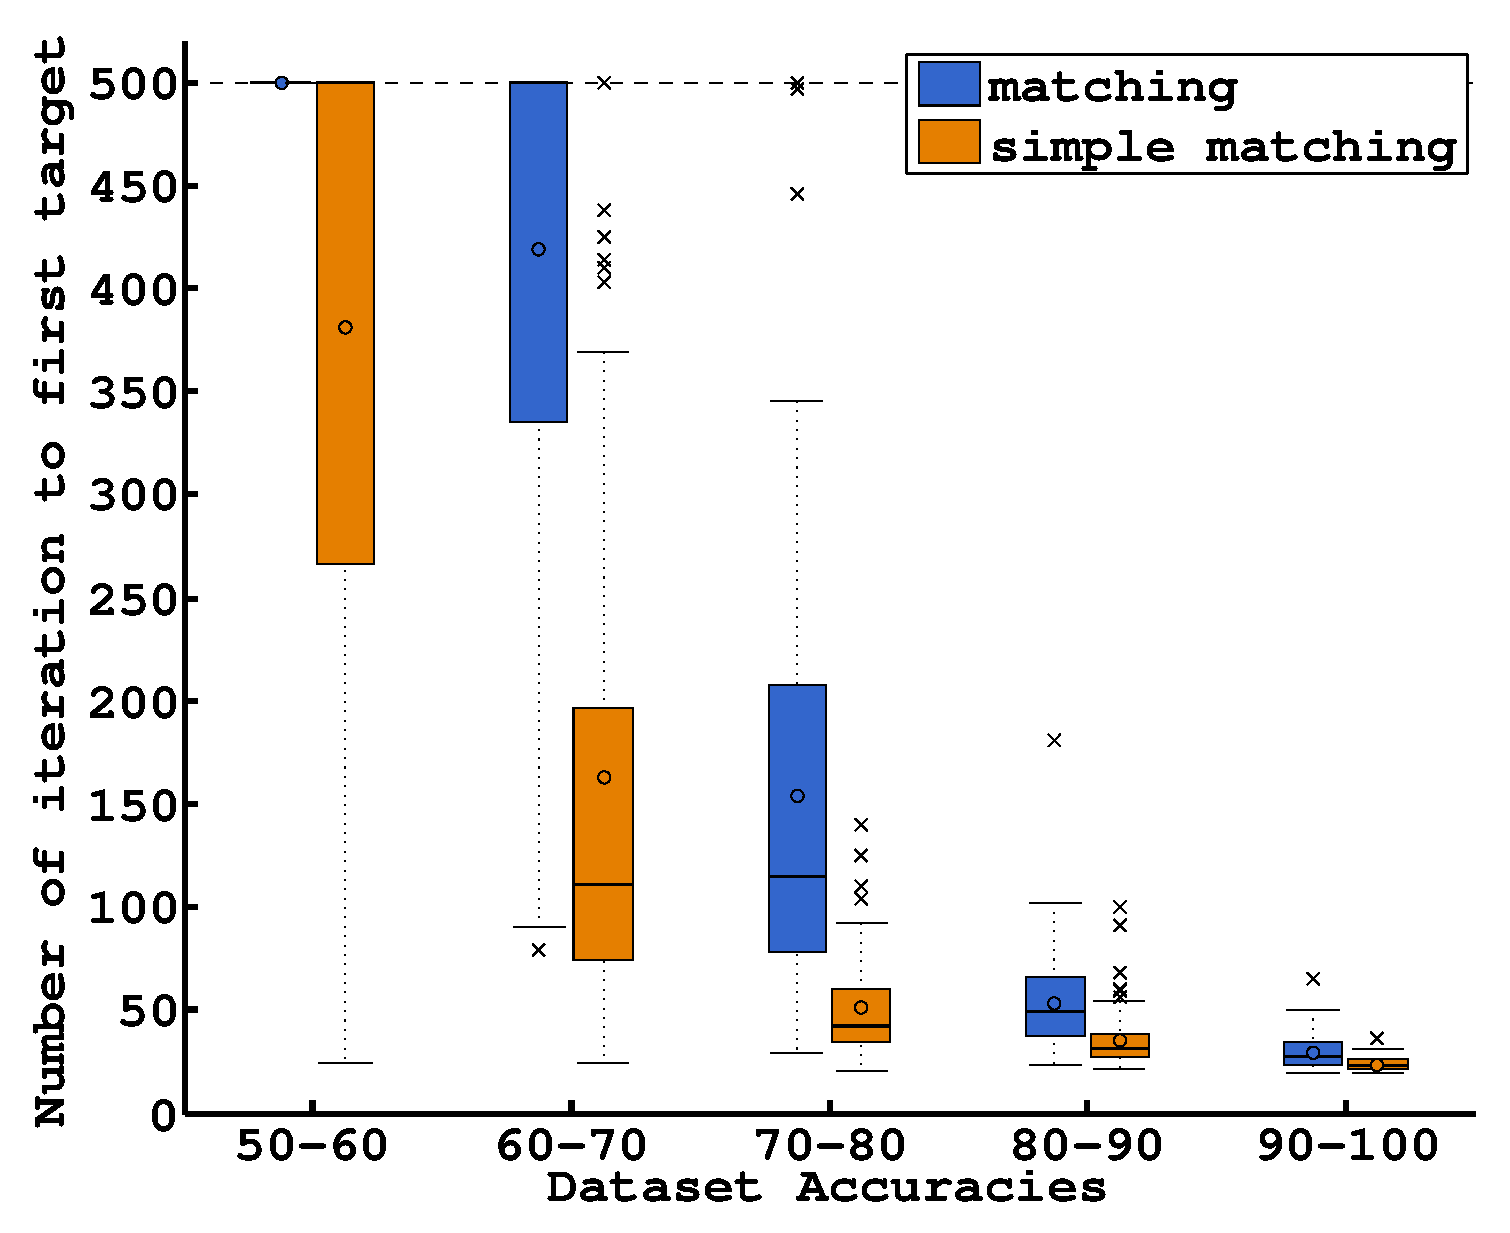
\includegraphics[width=\plotsize\columnwidth]{\imgpath/timefirst.eps}
\caption{Number of steps to complete the first task for all subjects in our online experiments. The results are plotted against the a posteriori computed 10-fold accuracy of our classifier on each subject EEG signals. The relation between data quality and the time to first task is in line with our simulated results shown in Figure~\ref{fig:timefirst_powermatching}. Note that the first target was evaluated correctly for every subject.}
\label{fig:timefirst_online}
\end{figure}

\subsubsection*{Extensions}

Dans un chapitre d'extension, nous traitons d'une multipte de problème et limitaiton immediate posé par l'utilisation de ce genre de système.

Nous montrons d'abord qu'il est possible d'utiliser le systeme dans des porblemes au espace detat continue. 

Nous ontron au chapitre que nous ne somme pas limité a définir un ensemble fini d'hypothès sur la tache.

Finalement nous montrons que la connaissance du protocole d'interaction a priori n;est pas non plus une limitation forte et le systeme peut detecter le bon protocole par l'interaction pratique avec l'utlisateur.

Enfin nous décrivons un preuve mathematique simple des fondement de notre methode ouvrant la voie à des guarantie plus grande sur la convergence et performance de nos algorthme


espace d'état continue

espace des taches continue

hypothèse sur le protocole d'interaction

preuve

\subsection*{Expèrience humain-humain}

Une question naturelle est de ce demander si une interaction aussi peu contrainte pourra fonctionner avec deux humains. Nous avons donc mis en place une experience de ce type avec deux humains devant intéragir par le biais d'une interface simple dont le sens des signaux était inconnue au départ pour les deux parties. 

Nous appelons l'utilisateur du qui appuie sur les boutons et connais la tàche, l'architecte. L'utlisateur qui observe les signaux et agit sur le monde est appelé le constructeur.

Il est intérressant de voir la construction dun language commun, non prévu au début

Une personne extèrieure à l'experience ne pourra pas comprendre ce qui ce passe en observant le résultat final de l'intéraction, sans connaitre l'historique.

\begin{figure}[!htbp]
\centering
\includegraphics[width=0.68\columnwidth]{\visualspng/humanexp/setup/setup_normal_video_one_column.png}
\caption{Schematic view of our experimental setup. An architect (bottom) and a builder (top) should collaborate in order to build the construction target while located in different rooms. The architect has a picture of the targeted construction, while the builder has access to the construction blocks. The communication between them is restricted. The architect only sees a top view of the builder's workspace and can communicate with the builder only though the use of 10 buttons which, when pressed, display symbols on a screen on the builder side.}
\label{fig:overviewsetup}
\end{figure}

\subsection*{Conclusion}

La vision dévellopé dans cette thèse est qu'il est possible pour une machine d'executé les souhait d'un utilisateur sans comprende la facon précise dont l'utisateur communique l'information. Plus concretmenet notre systeme n'a pas d'apriori sur le sens des mots et construit son modèle en interaction avec l'utilisateur sans jamais avoir access a une source sure d'information.

Au dela du challenge technique de l'auto-calibration, des questions d'utilisation pratique et d'acceptabilité eclose.

Comment les gens vont réagir au fait que la machine, le robot, ne soit plus apte immédiatement mais doivent apprendre le sens des signaux.
